\section{Introduction}
\paragraph{}
Consider the following missile intercept problem,
\begin{figure}[h]
	\centering
	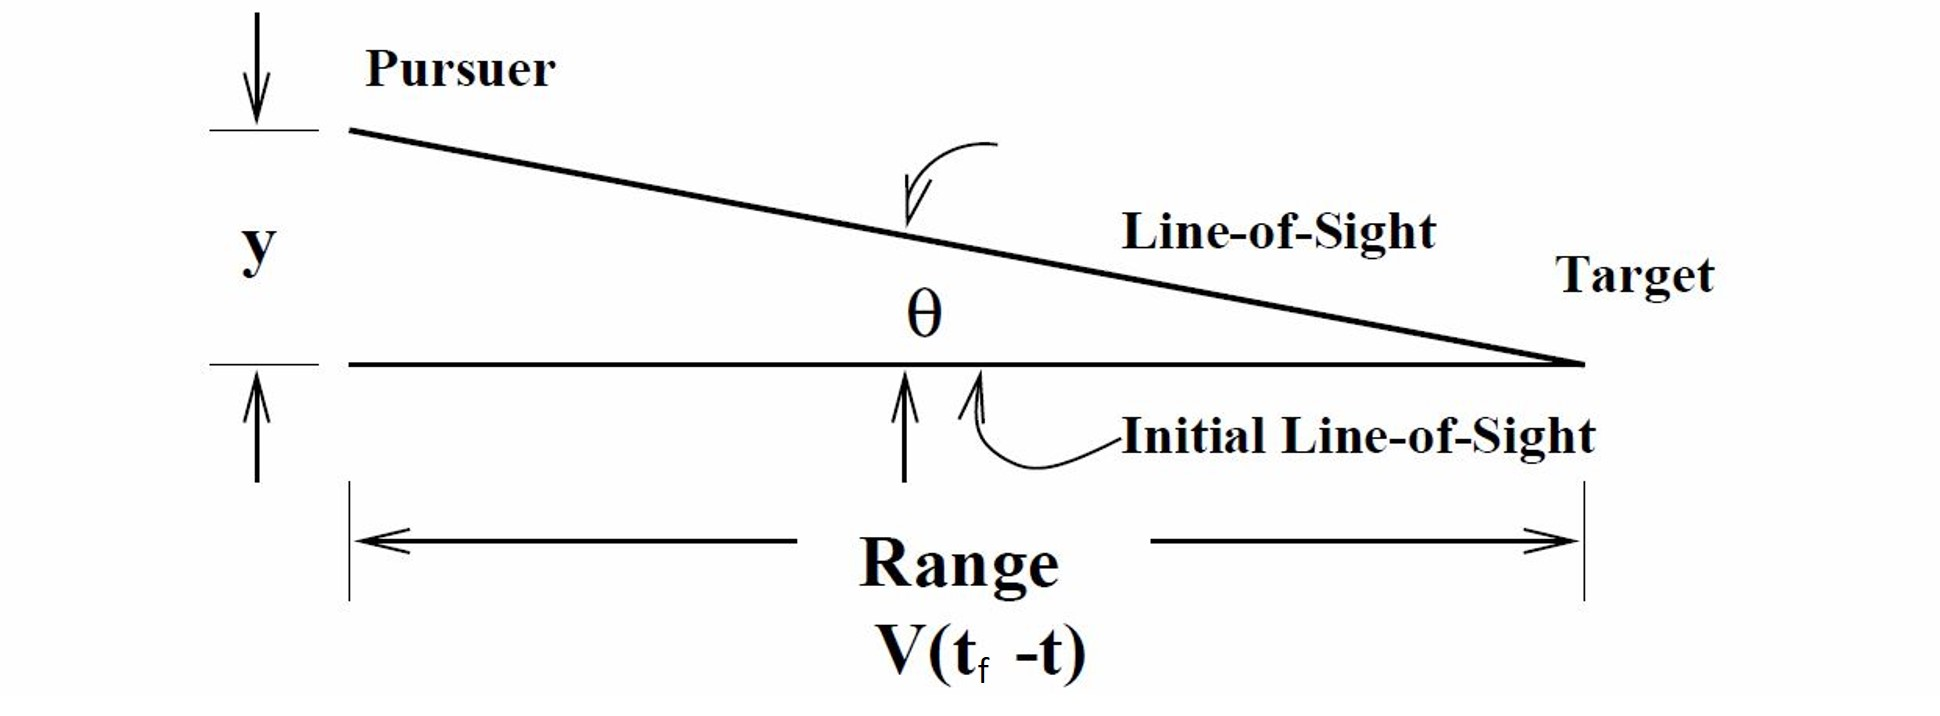
\includegraphics[width =1.1\textwidth]{pro.jpg}
	\caption{A Illustration of the Missile Intercept \cite{js}}
\end{figure}
\vspace{-18pt}
\paragraph{}
At starting time $t = 0$, the pursuer captures its target and start pursuing, i.e., narrowing the range. At terminal time $t = t_f$, it catches up with the target with horizontal distance $x = V(t_f - t) = 0$. To ensure the success of missile intercept, we need to minimize the vertical distance $y$ at time $t_f$. The dynamics of this problem are
\begin{equation}
	\begin{aligned}
		&\dot{y} = v,\\
		&\dot{v} = a_p -a_T,
	\end{aligned}
\end{equation}
\paragraph{}
where $a_p$, the missile acceleration, is known and assumed to be zero. The input $a_T$ is the target acceleration and is treated as a random forcing term with an exponential correlation,
\begin{align*}
&E[a_T] = 0,\\
&E[a_T(t)a_T(s)] = a_T^2e^{\frac{-|t-s|}{\tau}},
\end{align*}
\paragraph{}
where the scalar $\tau$ is the correlation time. The initial states are given as follows.
\begin{align*}
&E[y(t_0)] = 0, &E[v(t_0)] = 0,\\
&E[y(t_0)^2] = 0,  &E[y(t_0)v(t_0)]=0, & \qquad\qquad  E[v(t_0)^2] =\text{given}.
\end{align*}
\paragraph{}
The measurement $z$, consists of a line-of-sight angle, $\theta$. For $|\theta| \ll 1$,
\begin{align*}
\theta \approx \frac{y}{V_c(t_f-t)}.
\end{align*}
\paragraph{}
Also, it it assumed that $z$ is corrupted by a fading and scintillation noise so that
\begin{align*}
&z = \theta + n,\\
&E[n(t)] = 0, \\
&E[n(t)n(\tau)] = V\delta(t-\tau) = [R_1 + \frac{R_2}{(t_f-t)^2}]\delta(t-\tau).
\end{align*}
